\begin{table}[t]
\centering
\caption{Main Results on Effectiveness. We group the frameworks into \emph{Iterative} (utilize execution feedback to debug) and \emph{Single-Pass} (generate models directly). \textbf{Bold} indicates the best performance within each respective group. \methodname{} function best for single-pass generation and achieves performance highly comparable to fully iterative agents.}
% \begin{small} 
% \setlength{\tabcolsep}{4.5pt} 
\begin{tabular}{llc@{\hskip 12pt}cc@{\hskip 12pt}cc} 
\toprule
& & \multicolumn{3}{c}{\textbf{Single-Pass (No Execution)}} & \multicolumn{2}{c}{\textbf{Iterative (w/ Execution)}} \\
\cmidrule(lr){3-5} \cmidrule(lr){6-7}
\textbf{Model} & \textbf{Metric} & \textbf{\methodname{} (Ours)} & \textbf{OpenH-L} & \textbf{SWE-L} & \textbf{OpenH} & \textbf{SWE} \\ 
\midrule
\multirow{2}{*}{\textbf{GPT-5.2}} 
& $\text{Score}_{\text{beh}}$ & 0.87 $\pm$ 0.27 & \textbf{0.91 $\pm$ 0.23} & 0.00 $\pm$ 0.00 & 0.90 $\pm$ 0.24 & 0.82 $\pm$ 0.36 \\
& $\text{Score}_{\text{ope}}$ & 0.90 $\pm$ 0.20 & \textbf{0.95 $\pm$ 0.22} & 0.00 $\pm$ 0.00 & \textbf{0.95 $\pm$ 0.22} & 0.86 $\pm$ 0.36 \\
\midrule
\multirow{2}{*}{\textbf{GLM-4.7}} 
& $\text{Score}_{\text{beh}}$ & \textbf{0.75 $\pm$ 0.23} & \textbf{0.75 $\pm$ 0.27} & 0.56 $\pm$ 0.42 & \textbf{0.91 $\pm$ 0.09} & 0.70 $\pm$ 0.41 \\
& $\text{Score}_{\text{ope}}$ & \textbf{0.95 $\pm$ 0.24} & 0.90 $\pm$ 0.30 & 0.76 $\pm$ 0.44 & \textbf{1.00 $\pm$ 0.00} & 0.76 $\pm$ 0.44 \\
\midrule
\multirow{2}{*}{\textbf{Qwen3-30B}} 
& $\text{Score}_{\text{beh}}$ & 0.59 $\pm$ 0.32 & 0.60 $\pm$ 0.38 & \textbf{0.66 $\pm$ 0.24} & 0.61 $\pm$ 0.38 & \textbf{0.73 $\pm$ 0.29} \\
& $\text{Score}_{\text{ope}}$ & 0.82 $\pm$ 0.39 & 0.76 $\pm$ 0.44 & \textbf{0.95 $\pm$ 0.22} & 0.86 $\pm$ 0.35 & \textbf{0.90 $\pm$ 0.30} \\
\midrule
\multirow{2}{*}{\textbf{Llama-4-17B}} 
& $\text{Score}_{\text{beh}}$ & \textbf{0.31 $\pm$ 0.27} & 0.22 $\pm$ 0.30 & 0.24 $\pm$ 0.25 & 0.12 $\pm$ 0.23 & \textbf{0.28 $\pm$ 0.30} \\
& $\text{Score}_{\text{ope}}$ & \textbf{1.0 $\pm$ 0} & 0.43 $\pm$ 0.51 & 0.67 $\pm$ 0.48 & 0.28 $\pm$ 0.45 & \textbf{0.57 $\pm$ 0.51} \\
\bottomrule
\end{tabular}\label{tab:main_results}
% \end{small}
\end{table}

\section{Experiments}
\label{sec:experiments}

In this section, we evaluate the \methodname{} and several LLM-based software engineering agents. Our evaluation addresses three questions: (i) \emph{Effectiveness:} Can \methodname{} reliably synthesize correct world models? (ii) \emph{Efficiency:} How does the resource consumption (time and tokens) compare to iterative agents? (iii) \emph{Ablation:} How do strict DEVS formalism constraints impact the generation process, and how does our pipeline mitigate these challenges?

\subsection{Experimental Setup}

We conduct experiments using the benchmark we built in Section~\ref{sec:method_evaluation}. All local environments are executed on a CPU machine, interfacing with LLMs via API endpoints like OpenRouter. We report the $\text{Score}_{\text{ope}}$ and $\text{Score}_{\text{beh}}$. For efficiency, while token tracking can vary across different agent runtimes, so we use wall-clock time as a universal indicator of debugging stagnation.

For the main effectiveness evaluation, we compare \methodname{} against two open-source agentic frameworks: \texttt{OpenHands} \cite{wang2025openhandssoftwareagentsdk} and \texttt{SWE-Agent} \cite{yang2024sweagent}. We evaluate their Standard (Iterative) configs alongside their restricted Lite (Non-Iterative) variants to isolate the impact of execution feedback.

\subsection{Main Results}

\noindent\textbf{Effectiveness.}
Table~\ref{tab:main_results} reports the mean and standard deviation for $\text{Score}_{\text{ope}}$ and $\text{Score}_{\text{beh}}$. Across all models, \methodname{} achieves operational success rates comparable to fully iterative agents. It accomplishes this while operating entirely without code execution or debugging loops, suggesting that the structural blueprint provided by \plantree{} acts as a ``correct-by-construction'' guide.

The utility of our specification-driven approach is further highlighted when compared to the non-iterative baselines. Without execution feedback, unconstrained agents are highly susceptible to hallucination. By anchoring the generation to \plantree{}, \methodname{} maintains stable effectiveness in a single pass. 


% \begin{table}[h]
% \centering
% \caption{Timeout-aware Efficiency Comparison. We report Completion Rate (\%), Observed Tokens for successful runs, and Effective Tokens (which penalizes timeouts and failures).}
% \label{tab:efficiency}
% % \resizebox{\columnwidth}{!}{%
% \begin{tabular}{@{}llccc@{}}
% \toprule
% \textbf{Model} & \textbf{Framework} & \textbf{Comp. Rate} & \textbf{Observed Tokens (k)} & \textbf{Effective Tokens (k)} \\ \midrule
% \multirow{3}{*}{\textbf{GPT-5.2}} 
% & \textbf{\methodname{} (Ours)} & 90\% & \textbf{244 $\pm$ 125} & 697 $\pm$ 1435 \\
% & OpenHands & 95\% & 546 $\pm$ 694 & 758 $\pm$ 1184 \\
% & SWE-Agent & \textbf{100\%} & 320 $\pm$ 210 & \textbf{320 $\pm$ 210} \\ \midrule
% \multirow{3}{*}{\textbf{GLM-4.7}} 
% & \textbf{\methodname{} (Ours)} & 95\% & \textbf{152 $\pm$ 93} & \textbf{382 $\pm$ 1036} \\
% & OpenHands & \textbf{100\%} & 619 $\pm$ 432 & 619 $\pm$ 432 \\
% & SWE-Agent & \textbf{100\%} & 1976 $\pm$ 1032 & 1976 $\pm$ 1032 \\ \midrule
% \multirow{3}{*}{\textbf{Qwen3-30B}} 
% & \textbf{\methodname{} (Ours)} & 90\% & \textbf{211 $\pm$ 150} & \textbf{667 $\pm$ 1448} \\
% & OpenHands & 90\% & 765 $\pm$ 678 & 1169 $\pm$ 1427 \\
% & SWE-Agent & \textbf{100\%} & 1265 $\pm$ 743 & 1265 $\pm$ 743 \\ \midrule
% \multirow{3}{*}{\textbf{Llama-4-17B}} 
% & \textbf{\methodname{} (Ours)} & 76\% & 212 $\pm$ 146 & \textbf{1352 $\pm$ 2094} \\
% & OpenHands & 29\% & 80 $\pm$ 85 & 3594 $\pm$ 2278 \\
% & SWE-Agent & \textbf{95\%} & \textbf{26 $\pm$ 15} & 264 $\pm$ 1085 \\ \bottomrule
% \end{tabular}%
% % }
% \end{table}

% \noindent\textbf{Efficiency. }
% Iterative agents often fall into cycles of failed debugging, inflating both time and token usage. Table~\ref{tab:efficiency} outlines this difference. On GLM-4.7, \methodname{} reduces the token footprint by an order of magnitude compared to \texttt{SWE-Agent}. Even when factoring in effective token penalties for compilation failures, \methodname{} remains substantially more efficient. This stems from structural decoupling: instead of feeding massive error logs back into a monolithic context window, the LLM processes localized, independent contracts in parallel.

% \begin{table}[t]
% \centering
% \caption{Efficiency and Parallelism. We report Success Rate (SR), Success Time (ST, average latency of successful runs in seconds), and Penalized Time (PT, system-level latency penalizing non-terminating loops in seconds). \methodname{} achieves significantly lower effective latency, bypassing the sequential bottlenecks of standard agents.}
% \label{tab:efficiency}
% \resizebox{\linewidth}{!}{
% \setlength{\tabcolsep}{4pt} 
% \begin{tabular}{@{} l ccc ccc ccc ccc @{}} 
% \toprule
% \multirow{2}{*}{\textbf{Method}} & \multicolumn{3}{c}{\textbf{GPT-5.2}} & \multicolumn{3}{c}{\textbf{GLM-4.7}} & \multicolumn{3}{c}{\textbf{Qwen3-30B}} & \multicolumn{3}{c}{\textbf{Llama-4-17B}} \\
% \cmidrule(lr){2-4} \cmidrule(lr){5-7} \cmidrule(lr){8-10} \cmidrule(lr){11-13}
% & SR $\uparrow$ & ST $\downarrow$ & PT $\downarrow$ & SR $\uparrow$ & ST $\downarrow$ & PT $\downarrow$ & SR $\uparrow$ & ST $\downarrow$ & PT $\downarrow$ & SR $\uparrow$ & ST $\downarrow$ & PT $\downarrow$ \\ 
% \midrule
% \textbf{SWE} 
% & 85.7\% & \textbf{517.6} & 1015.1 
% & 76.2\% & 351.7 & 1220.3 
% & 90.5\% & 633.1 & 953.7 
% & 57.1\% & \textbf{62.7} & 1750.1 \\
% \textbf{OpenHands} 
% & 95.2\% & 777.4 & 930.8 
% & \textbf{100.0\%} & \textbf{105.9} & \textbf{105.9} 
% & 90.5\% & 417.1 & 758.3 
% & 23.8\% & 82.9 & 3067.3 \\
% \textbf{\methodname{} (Ours)} 
% & \textbf{100.0\%} & 555.9 & \textbf{555.9} 
% & \textbf{100.0\%} & 955.6 & 955.6 
% & \textbf{95.8\%} & \textbf{377.5} & \textbf{528.5} 
% & \textbf{100.0\%} & 197.9 & \textbf{197.9} \\
% \bottomrule
% \end{tabular}
% }
% \end{table}

% \noindent\textbf{Efficiency }
% Table~\ref{tab:efficiency} evaluates efficiency using three metrics: \emph{Success Rate}, \emph{Success Time} (average duration of successful runs), and \emph{Penalized Time} (system-level duration incorporating maximum timeout penalties for non-terminating loops). While iterative agents occasionally achieve low \emph{Success Times} on simple scenarios, their \emph{Penalized Times} inflate drastically due to frequent non-terminating loops. For example, Llama-4-17B on \texttt{OpenHands} records a \emph{Success Time} of only 82.9s, but its low \emph{Success Rate} (23.8\%) drives the \emph{Penalized Time} to a prohibitive 3067.3s. 

% In contrast, \methodname{} avoids sequential debugging dependencies entirely. By explicitly assigning independent interface contracts via \plantree{} in Stage 1, the framework can synthesize all atomic components in parallel during Stage 2. This concurrent, forward-pass construction eliminates non-terminating loops, resulting in highly predictable and competitive \emph{Penalized Times}.

\begin{figure}[t]
    \centering
    % \columnwidth 或 \linewidth
    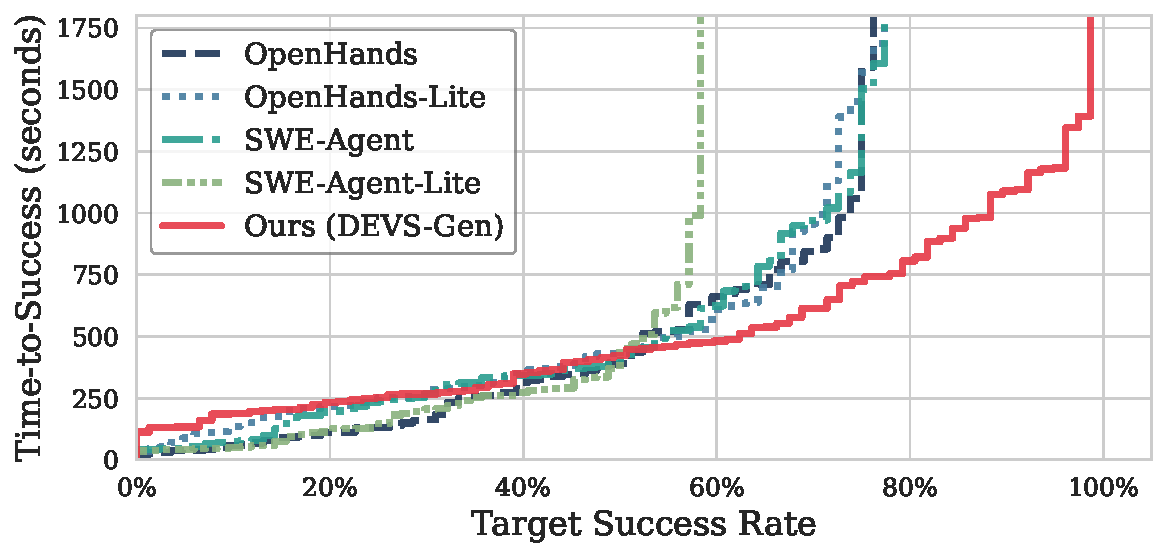
\includegraphics[width=0.7\columnwidth]{imgs/tts_cdf_all.pdf}
    \caption{Time-to-Success distribution across all evaluated models. The x-axis represents the cumulative success rate, and the y-axis indicates the wall-clock time required to achieve it. While baseline agents show low initial latency, they hit a vertical wall before reaching an $80\%$ success rate due to non-terminating debugging cycles. In contrast, \methodname{} translates computation time into continuous task completion, reliably scaling to near $100\%$ success.}
    \label{fig:tts_cdf}
\end{figure}
\noindent\textbf{Efficiency.} 
Relying on metrics like average execution time to evaluate efficiency introduces severe bias, as the timeouts are not properly reflected. So we presents the Time-to-Success distribution in Figure~\ref{fig:tts_cdf}, illustrating the time cost required to achieve a target success rate over all tested models.

The distribution reveals a critical bottleneck for standard agents. While frameworks like \texttt{OpenHands} and \texttt{SWE-Agent} exhibit competitive latency on some simple tasks, they rapidly hit a vertical wall. They fall into non-terminating debugging cycles and fail to surpass an $80\%$ success threshold, regardless of the time budget. 

In contrast, \methodname{} demonstrates highly predictable scaling. Although constructing the \plantree{} incurs a minor initial overhead, this structural decoupling enables parallel synthesis. It translates computation time into continuous task completion, pushing its success rate toward $100\%$.

\subsection{Ablation: Framework Constraints and Cognitive Load}
\label{sec:ablation_xdevs}

The DEVS formalism provides a modular architecture for complex simulators, but directly enforcing its strict structural rules imposes a heavy cognitive load on LLMs. To evaluate this, we compare three non-iterative setups: unconstrained direct prompting \texttt{single} and constraint-forced direct prompting \texttt{single-xdevs} (forced to use \texttt{xdevs.py}, equipped with necessary knowledge of the framework) to establish the baseline cognitive load of the DEVS formalism, comparing them against \methodname{}.

Table~\ref{tab:ablation_xdevs} reports the performance on a representative Large (GLM-4.7) and Small (Qwen3-30B) model. LLMs achieve robust baseline scores when generating free-form, monolithic scripts (\texttt{single}). However, enforcing highly structured DEVS semantics (\texttt{single-xdevs}) causes significant drops. This indicates that simultaneously managing global architectural routing and local formalism syntax overwhelms the model's context capacity.

\methodname{} mitigates this structural complexity. By pre-solving the architectural routing and assigning interface contracts via \plantree{}, the pipeline allows the LLM to focus entirely on localized logic. Consequently, \methodname{} overcomes the cognitive penalty of the formal constraints and surpasses the unconstrained baselines (e.g., improving $\text{Score}_{\text{ope}}$ to 0.95 on GLM-4.7).

\begin{table}[h]
\centering
\caption{Ablation on Framework Constraints. We report $\text{Score}_{\text{ope}}$ and $\text{Score}_{\text{beh}}$. Directly enforcing strict structural rules (\texttt{single-xdevs}) causes a performance drop across both metrics compared to free-form coding (\texttt{single}). \methodname{} utilizes the \plantree{} scaffold to absorb this complexity, surpassing the unconstrained baselines.}
\label{tab:ablation_xdevs}
\begin{tabular}{@{}lcccc@{}}
\toprule
& \multicolumn{2}{c}{\textbf{GLM-4.7 (Large)}} & \multicolumn{2}{c}{\textbf{Qwen3-30B (Small)}} \\
\cmidrule(lr){2-3} \cmidrule(lr){4-5}
\textbf{Setup} & \textbf{$\text{Score}_{\text{ope}}$ $\uparrow$} & \textbf{$\text{Score}_{\text{beh}}$ $\uparrow$} & \textbf{$\text{Score}_{\text{ope}}$ $\uparrow$} & \textbf{$\text{Score}_{\text{beh}}$ $\uparrow$} \\ \midrule
\texttt{single} (Unconstrained) & 0.74 & 0.57 & 0.74 & 0.51 \\
\texttt{single-xdevs} (Strict \texttt{xdevs}) & 0.45 ($\downarrow$ 0.29) & 0.30 ($\downarrow$ 0.27) & 0.66 ($\downarrow$ 0.08) & 0.43 ($\downarrow$ 0.08) \\
\midrule
\rowcolor{gray!15}
\textbf{\methodname{} (Ours)} & \textbf{0.95} ($\uparrow$ \textbf{0.50}) & \textbf{0.74} ($\uparrow$ \textbf{0.44}) & \textbf{0.82} ($\uparrow$ \textbf{0.16}) & \textbf{0.59} ($\uparrow$ \textbf{0.16}) \\ \bottomrule
\end{tabular}
\end{table}

\subsection{Ablation Study: Scalability and Parallel Synthesis}
\label{sec:ablation}

A key architectural advantage of \methodname{} is its ability to decouple the synthesis process, which permits the parallel execution of structural planning and atomic model implementation. Predicated on the standard modeling practice where a coupled model aggregates at least two subcomponents (i.e., a branching factor $b \ge 2$), the depth of the system hierarchy grows logarithmically with the total number of components $N$. Consequently, the theoretical synthesis latency is governed by the critical path of this hierarchy rather than the sequential accumulation of all tasks. This structural property reduces the time complexity from linear $O(N)$ (characteristic of serial approaches), to logarithmic $O(\log N)$.

To validate this, we conducted an ablation study using GPT-5.2 on the \methodname{} framework, comparing the wall-clock time of serial execution versus parallel execution. Figure~\ref{fig:parallel_ablation} reports the speed-up across the two stages.

% \begin{itemize}[leftmargin=*]
\textbf{Structural Planning Stage.} Theoretically, the recursive planning algorithm allows independent branches of the system hierarchy to be decomposed concurrently. However, as observed in Figure~\ref{fig:parallel_ablation}, the empirical speedup is modest. This is primarily due to the scale of our current benchmark scenarios: the system hierarchies are relatively shallow, meaning the overhead of network requests and thread management outweighs the benefits of parallelizing the lightweight component classification tasks. We expect this speedup to become significant only in much larger, deeply nested systems.
    
\textbf{Behavioral Synthesizing Stage.} The acceleration is substantial, achieving a $\sim 4.7\times$ speedup. Since atomic models (leaf nodes) encapsulate the bulk of the complex logic (state transitions and logic implementation), their generation is the computational bottleneck. Our framework successfully isolates these tasks, allowing them to be synthesized simultaneously. 
% \end{itemize}

This result proves the scalability of \methodname. While standard agentic loops face super-linear growth in time and context costs as system complexity increases, our modular approach ensures that the synthesis time grows logarithmically, making it feasible for large-scale world modeling.

\begin{figure}[h]
    \centering
    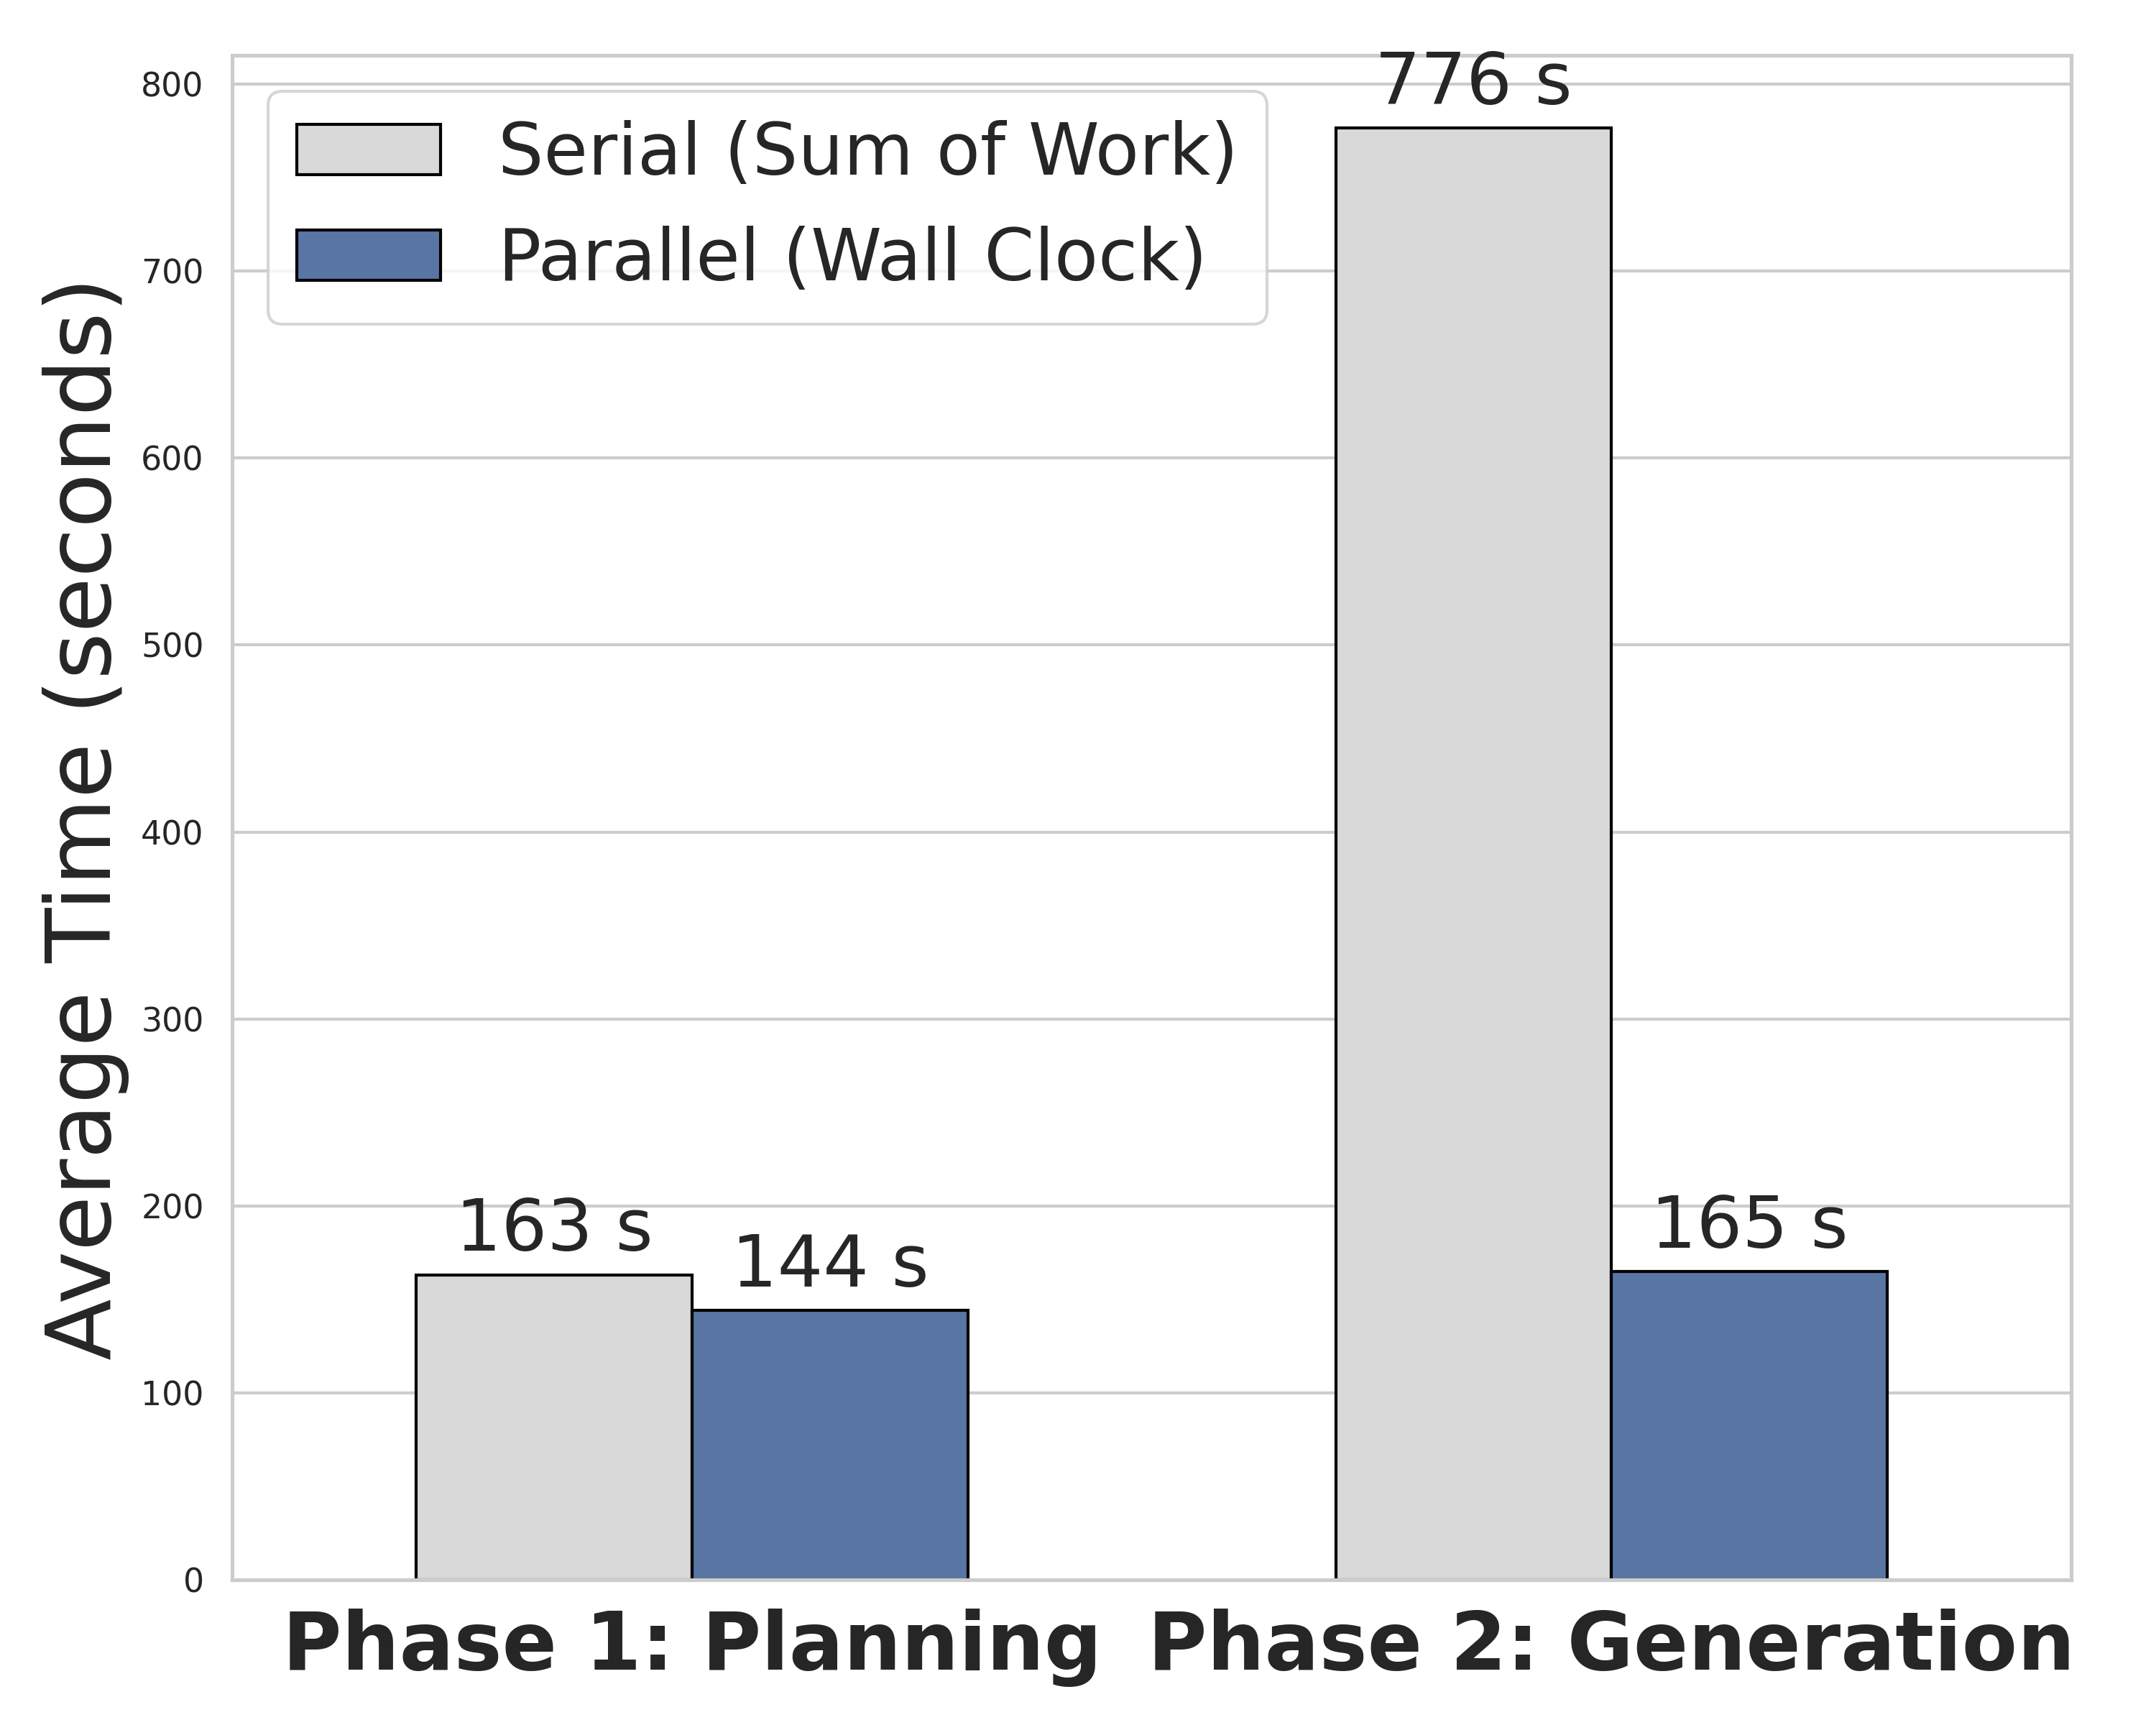
\includegraphics[width=0.45\columnwidth]{imgs/ablation_parall.png}
    \caption{Ablation study on synthesis latency (using GPT-5.2). The chart compares the wall-clock time required for the Planning and Generation phases under serial and parallel execution modes. While the acceleration in the Planning phase is limited by the current benchmark scale, the Generation phase achieves a $4.7\times$ speedup, validating the scalability of the approach.}
    \label{fig:parallel_ablation}
\end{figure}